\chapter{الگوریتم بهینه‌سازی چند هدفه \lr{REAMRK}}
این فصل ابتدا به مفاهیم و تعاریف بهینه‌سازی چند هدفه و سپس به
 به تبدیل الگوریتم بهینه‌سازی تک هدفه \lr{REMARK}
به چند هدفه پرداخته است.


\section{بهینه‌سازی چند هدفه}

بهینه سازی چند هدفه، حوزه‌ای از تصمیم‌گیری چند معیاری محسوب می‌شود. بهینه‌سازی چند هدفه با مسائل بهینه‌سازی ریاضیاتی سروکار دارد که در آن‌ها نیاز است بیش از یک تابع هدف، به طور همزمان، بهینه‌سازی شوند. بهینه‌سازی چند هدفه با نام‌های دیگری نظیر برنامه ریزی چند هدفه\LTRfootnote{Multi-Objective Programming}، بهینه‌سازی برداری\LTRfootnote{Vector OPtimization}، بهینه‌سازی چند معیاری\LTRfootnote{Multi-Criteria Optimization}، بهینه‌سازی چند مشخصه‌ای\LTRfootnote{Multi-Attribute Optimization} یا بهینه‌سازی پارتو\LTRfootnote{Pareto Optimization} نیز شناخته می‌شود.


روش‌های بهینه‌سازی چند هدفه در بسیاری از شاخه‌های علوم و مهندسی به کار گرفته شده‌اند و زمانی مورد استفاده قرار می‌گیرند که برای رسیدن به تصمیمات بهینه در سیستم، نیاز است میان دو یا چند هدف متناقض موازنه\LTRfootnote{Trade-off} برقرار شود. بدون شک در بسیاری از کاربردهای مهندسی، طراحان فرایند و سیستم‌های مهندسی بر اساس اهداف متناقض، تصمیم‌گیری می‌کنند. به عنوان نمونه، در فرایند طراحی هواپیما، علاوه بر اینکه هدف مهندسان طراحی خودرویی است که عملکرد\LTRfootnote{Performance} حداکثری داشته باشد، به طور همزمان، به دنبال طراحی هواپیمایی هستند که کمترین میزان آلایندگی و مصرف سوخت را داشته باشد. شکل
\ref{fig:multi_space}
در فضای دو بعدی دو تابع هدف را نشان داده است.
\begin{figure}[H]
	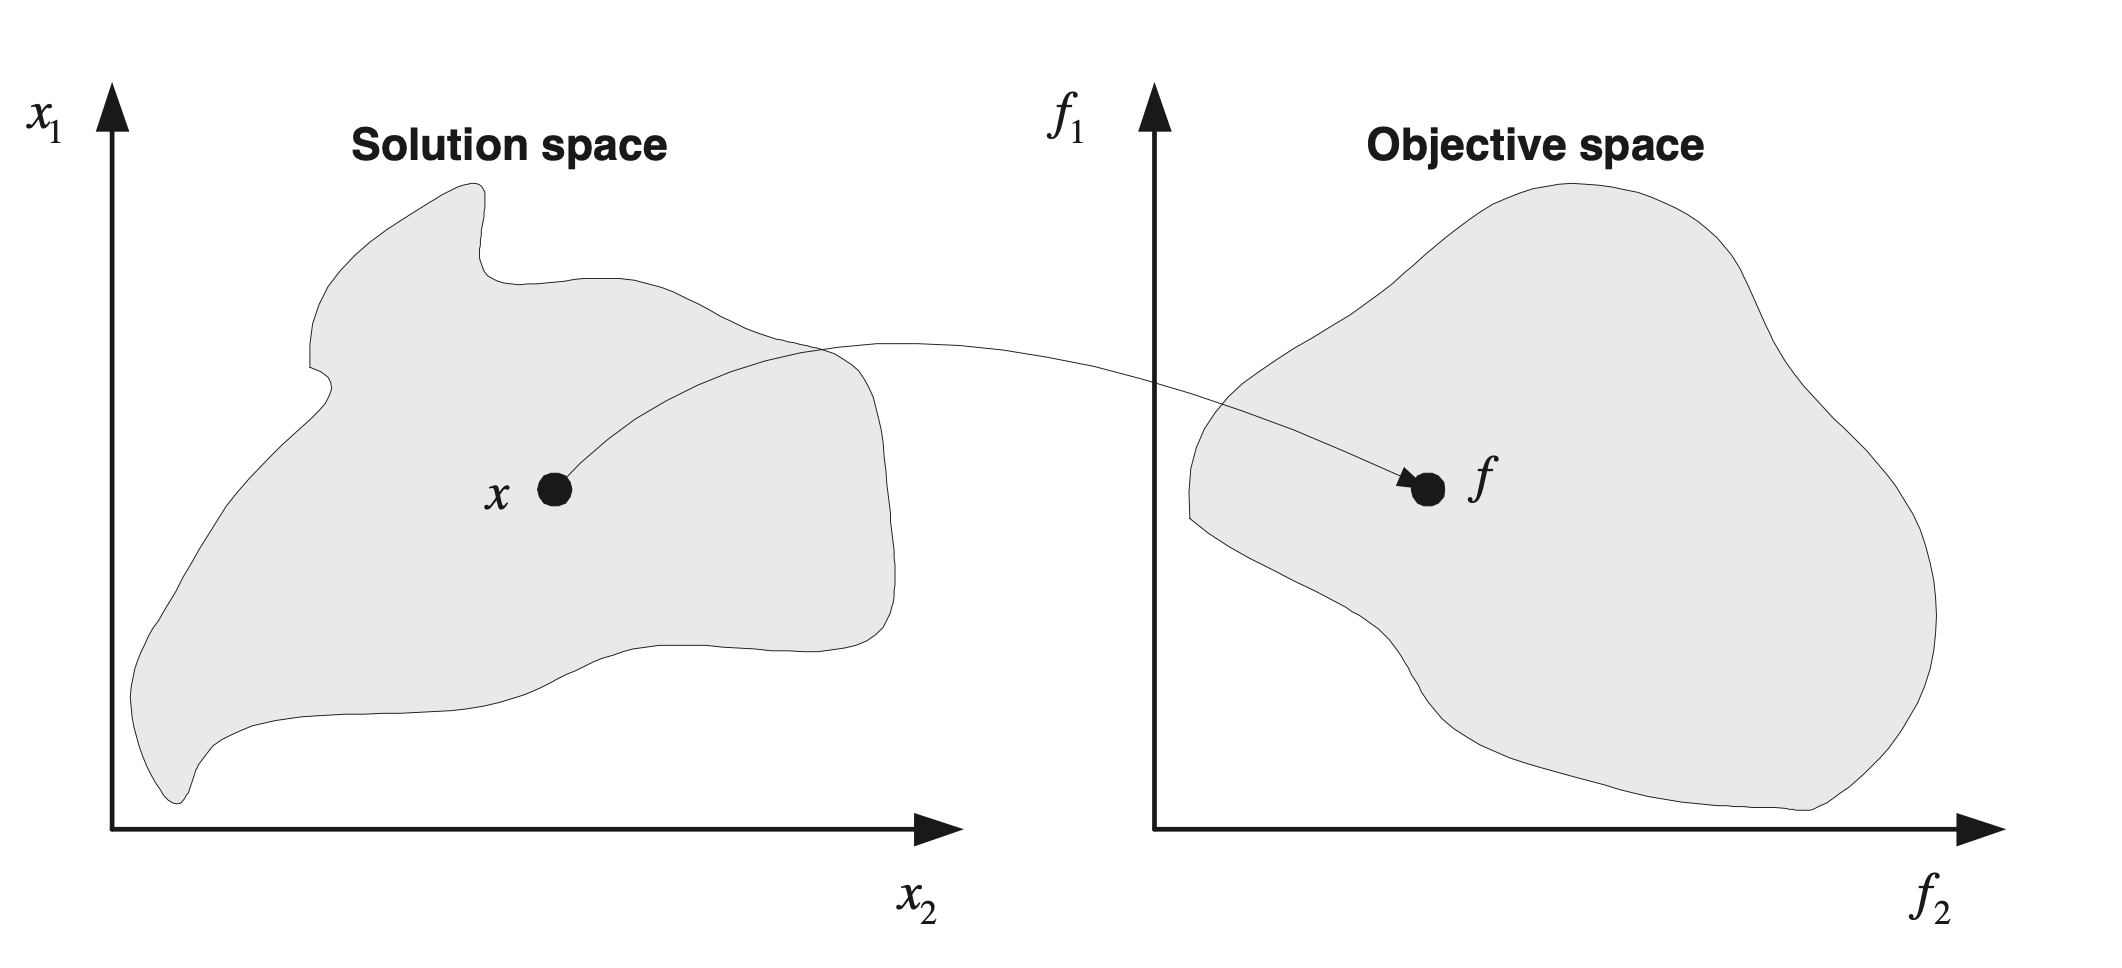
\includegraphics[width=16cm]{../Figure/multi-objective/multi_space.png}
	\centering
	\caption{تصویری از نگاشت بین فضای حل و فضای هدف
	\cite{10635_16724}}
\label{fig:multi_space}
\end{figure}


در این مورد و موارد مشابه، از آنجایی که بیش از یک تابع هدف باید مورد بررسی قرار بگیرد، نیاز است تا به کارگیری روش‌های بهینه‌سازی چند هدفه مورد بررسی قرار بگیرد. مهم‌ترین ویژگی در چنین روش‌هایی این است که با به‌کارگیری مدل‌های بهینه‌سازی چند هدفه، بیش از یک جواب کاندید (یک جواب ممکن برای مسأله مورد نظر) در اختیار طراحان و مهندسان سیستم قرار گرفته می‌شود؛ هر یک از این جواب‌ها، موازنه میان توابع هدف مختلف را نمایش خواهند داد.

مفهومی به نام جواب نامسلط\LTRfootnote{Non-Dominated} در سیستم‌های حل مسائل بهینه سازی چند هدفه وجود دارد. در صورتی به یک جواب کاندید برای مسأله بهینه سازی چند هدفه، جواب نامسلط گفته می‌شود که بهبود مقادیر تولید شده توسط یک یا چند تابع هدف از این مسأله (از طریق قرار دادن جواب کاندید در توابع هدف و تولید مقادیر خروجی)، سبب کاهش کیفیت مقادیر تولید شده توسط دیگر توابع هدف همان مسأله شود. به چنین جواب‌هایی، بهینه پارتو\LTRfootnote{Pareto Optimal} گفته می‌شود. بدون در اختیار داشتن اطلاعات اضافی، تمامی جواب‌های بهینه پارتو به یک اندازه خوب هستند و با یکدیگر برابر در نظر گرفته می‌شوند.

\section{مفاهیم و نظریه}

\subsection{بهینگی پارتو}


به مفهوم تعریف جواب‌های یک مسأله بهینه‌سازی چند هدفه، بهینگی پارتو \LTRfootnote{Pareto Optimality} گفته می‌شود. در صورتی به نقطه 
$x^*$
در فضای طراحی مسأله
$(S)$
بهینه پارتو گفته می‌شود که در مجموعه 
$S$
نقطه دیگری وجود نداشته باشد که باعث کمینه‌سازی حداقل یکی از توابع هدف موجود در مسأله بهینه سازی چند هدفه و به طور همزمان، افزایش مقدار یک تابع هدف دیگر شود.
\begin{equation}
	f_i(x) \leq f_i(x^*) \quad \forall i
\end{equation}

\subsection{بهینه پارتوی ضعیف}
در نقاط بهینه پارتوی ضعیف\LTRfootnote{Weak Pareto Optimality}، این امکان وجود دارد که با بهینه‌سازی برخی از توابع هدف مسأله، کیفیت جواب‌های تولید شده توسط دیگر توابع هدف کاهش پیدا نکند.
به نقطه 
$x^*$
در فضای طراحی مسأله ($S$) بهینه پارتوی ضعیف گفته می‌شود که نقطه دیگری مانند 
$x \in S$
وجود نداشته باشد، به طوری که:
\begin{equation}
	f_i(x) < f_i(x^*) \quad \forall i
\end{equation}


\subsection{نقاط مسلط و نامسلط}
بردار متشکل از توابع هدف 
$f^*=f(x^*) \in Z$
نامسلط\LTRfootnote{Non-Dominated} شناخته می‌شود، اگر و تنها اگر، بردار دیگری نظیر 
$f\in Z$
وجود نداشته باشد، به طوری که:
\begin{equation}
	f_i \leq f_i^*\quad \forall i \textrm{  \lr{and}  } f_i < f_i^* \text{\lr{  for at least one }} i
\end{equation}

در غیر این صورت، بردار 
$f^*$
مسلط\LTRfootnote{Dominated} شناخته می‌شود. به طور کلی، بهینگی پارتو به هر همه‌ی فضاهای مسئله اشاره دارد.